\documentclass[a4paper,12pt]{report}
% \usepackage{styles/fbe_tez}
\usepackage[utf8]{inputenc}
\renewcommand{\labelenumi}{(\roman{enumi})}
\usepackage{amsmath, amsthm, amssymb}
\usepackage[bottom]{footmisc}
\usepackage{cite}
\usepackage{url}
\usepackage{graphicx}
\usepackage{longtable}
\usepackage{booktabs}
\usepackage{array}
\graphicspath{{figures/}{../tests/results/}}

\usepackage{multirow}
\usepackage{subfigure}
\usepackage{algorithm}
\usepackage{algorithmic}

\begin{document}

% Title Page
\title{CMPE 492 \\ MuJoCo-Based Autonomous Junction Simulation \\ \large Midterm Report}
\author{
Taha Ensar Kukul\\
\\ \\
Advisor: \\
Doğan Ulus
}
\date{}
\maketitle{}
\pagenumbering{roman}
\tableofcontents

% ─────────────────────────────────────────────────────────────────────────────
\chapter{INTRODUCTION}
\pagenumbering{arabic}

\section{Broad Impact}

Automation is rapidly advancing across many fields, and transportation is no
exception. Autonomous vehicles (AVs) have emerged as one of the most significant
developments in this space, with the potential to improve road safety, reduce
traffic congestion, and transform urban mobility. However, developing and
validating AV algorithms through physical testing is costly in terms of both
time and resources. Simulation environments offer a practical alternative,
enabling researchers to test and iterate on algorithms safely and efficiently.

One particularly challenging scenario for autonomous vehicles is navigating road
junctions, where complex multi-agent interactions and dynamic traffic conditions
demand robust decision-making. Accurate simulation of such scenarios requires
not only a realistic environment but also a physically faithful vehicle model.
A simulation that captures the true dynamic behaviour of the vehicle under test
is essential for producing results that remain meaningful beyond the virtual
environment.

This project addresses that need by implementing a mathematically accurate
digital twin of EDGAR — the research autonomous vehicle developed by the
Technical University of Munich (TUM) — within the MuJoCo physics simulation
framework, and deploying it in a junction simulation scenario. By grounding the
simulation in validated physical parameters and testing the model against the
vehicle's published performance specifications, this work aims to provide a
reliable foundation for studying autonomous intersection management strategies.

\section{Motivation for Vehicle Modeling}

A fundamental challenge in autonomous vehicle simulation is ensuring that the
simulated vehicle behaves like its real-world counterpart. Many simulation
frameworks treat vehicles as point masses or as kinematic agents that follow
predefined trajectories, without modelling tire forces, mass distribution, or
actuator dynamics. While such simplifications may be acceptable for high-level
traffic flow studies, they are inadequate for evaluating precise control
strategies where braking distances, turning radii, and longitudinal acceleration
envelopes are critical.

Modelling a vehicle accurately in a physics simulation requires defining its
geometry, mass distribution, and dynamic properties in a way that is faithful
to the physical system. For an autonomous vehicle research platform such as
EDGAR, this means reproducing the same mathematical constraints that appear in
the vehicle's onboard motion planner — maximum steering angles, acceleration and
deceleration limits, and the kinematic turning geometry. When the simulated
vehicle respects these constraints, experiments conducted in simulation can
produce results that are directly comparable to real-world trials and compatible
with planning algorithms designed for the actual vehicle.

This project implements the EDGAR vehicle model in the MuJoCo physics engine
and validates it against EDGAR's published specification to confirm that the
simulation faithfully reproduces the vehicle's physical capabilities.

\section{Ethical Considerations}

Autonomous vehicle research carries ethical responsibilities related to public
safety. Simulation-based development helps address these concerns by allowing
algorithms to be tested and refined extensively before any deployment. Physical
road testing of unvalidated AV software poses risks to both occupants and the
public. By adopting high-fidelity simulation, this project follows a
safety-first development approach; any decision-making algorithms developed here
are intended for research purposes only and would require thorough additional
validation before real-world application.

% ─────────────────────────────────────────────────────────────────────────────
\chapter{PROJECT DEFINITION AND PLANNING}

\section{Project Definition}

The primary goal of this project is to develop a MuJoCo-based simulation
environment in which one or more autonomous vehicles navigate a four-way road
junction without collisions and without manual control or traffic lights. The
project has two distinct layers: first, implementing a physically accurate
vehicle model that faithfully replicates the dynamics of the EDGAR autonomous
vehicle; and second, deploying that model in a junction scenario and designing
decision-making mechanisms that allow multiple vehicles to cross safely.

EDGAR was selected because TUM has published detailed mathematical parameters
for it as part of their open autonomous driving research ecosystem. This
provides a concrete, verifiable specification against which the simulation can
be validated, rather than relying on arbitrary or hypothetical vehicle data.

\section{Project Planning}

The project is organised into four sequential phases:

\begin{enumerate}
  \item \textbf{Phase 1 — EDGAR Vehicle Modelling:} Implement the EDGAR vehicle
        in MuJoCo from scratch using the vehicle's published digital twin
        specifications. Implement steering, throttle, and brake actuators.
        Validate the model against the vehicle's published geometric and dynamic
        performance parameters.

  \item \textbf{Phase 2 — Road and Junction Modelling:} Construct a four-way
        intersection environment in MuJoCo using geometric primitives and mesh
        assets. Ensure proper collision detection between vehicles and the
        environment.

  \item \textbf{Phase 3 — Multi-Vehicle Scenario:} Introduce multiple vehicle
        instances approaching the intersection from different directions and
        define arrival timing scenarios.

  \item \textbf{Phase 4 — Decision Mechanisms:} Implement and compare at least
        two intersection-crossing strategies (e.g., a fixed priority rule and a
        time-to-collision based policy), and evaluate them using performance
        metrics including average waiting time, collision count, and intersection
        throughput.
\end{enumerate}

At the time of this midterm report, Phase~1 has been completed. The EDGAR
vehicle model is implemented in MuJoCo and has been validated against the
vehicle's published specifications.

\subsection{Project Timeline}

\begin{table}[h]
\centering
\caption{Project phase timeline and current status.}
\begin{tabular}{|c|l|l|}
\hline
\textbf{Phase} & \textbf{Description} & \textbf{Status} \\ \hline
1 & EDGAR vehicle modelling and validation    & \textbf{Completed} \\ \hline
2 & Junction environment construction         & In progress        \\ \hline
3 & Multi-vehicle scenario                    & Planned            \\ \hline
4 & Decision mechanisms and evaluation        & Planned            \\ \hline
\end{tabular}
\label{table:timeline}
\end{table}

\subsection{Success Criteria}

The Phase~1 success criteria are:
\begin{itemize}
  \item The simulated vehicle's geometry (dimensions, wheelbase, track width,
        CG height) matches EDGAR's published specifications within a 5\%
        tolerance.
  \item The simulated vehicle sustains a longitudinal acceleration of at least
        $2.5\ \text{m/s}^2$ in the $40$–$100\ \text{km/h}$ speed range under
        full throttle.
  \item The simulated vehicle achieves a peak deceleration of at least
        $3.5\ \text{m/s}^2$ when full braking is applied from $40\ \text{km/h}$.
  \item The steering system reaches the commanded angle and the resulting turning
        radius is consistent with the kinematic bicycle model prediction.
\end{itemize}

The overall project success criterion is a functional, collision-free
multi-vehicle junction crossing scenario with at least two decision mechanisms
implemented and compared quantitatively.

\subsection{Risk Analysis}

\begin{table}[h]
\centering
\caption{Risk analysis.}
\begin{tabular}{|p{5.2cm}|l|p{5.8cm}|}
\hline
\textbf{Risk} & \textbf{Severity} & \textbf{Mitigation} \\ \hline
MuJoCo numerical instability at large forces & Medium &
  Tune timestep and damping coefficients iteratively. \\ \hline
Ackermann constraint linearisation error at large steering angles & Low &
  Validated by steering test; acceptable for urban speed range. \\ \hline
Junction geometry difficult to build in MuJoCo from scratch & Medium &
  Use mesh assets from external open-source repositories. \\ \hline
Multi-vehicle coordination more complex than anticipated & Medium &
  Reduce scope to simpler decision rules if required. \\ \hline
\end{tabular}
\label{table:risks}
\end{table}

% ─────────────────────────────────────────────────────────────────────────────
\chapter{RELATED WORK}

\section{Vehicle Dynamics Modelling}

Selecting the appropriate level of vehicle model fidelity is a fundamental
decision in any vehicle simulation study. The literature offers a range of
modelling approaches, each making different trade-offs between accuracy and
computational complexity \cite{rajamani2012}.

\subsection{Kinematic Bicycle Model}

The kinematic bicycle model, also called the single-track kinematic model, is
the simplest widely used vehicle representation. It collapses the two front
wheels into one and the two rear wheels into one, treating the vehicle as a
single-track system. The model assumes that no lateral tyre slip occurs, which
makes it valid at low speeds or in scenarios where tyre forces remain well below
the friction limit.

Taking the rear axle as the reference point, with vehicle heading $\psi$,
forward speed $v$, front-wheel steering angle $\delta$, and wheelbase $L$, the
kinematic equations of motion are:

\begin{align}
\dot{x}    &= v \cos\psi                        \label{eq:bm_x} \\
\dot{y}    &= v \sin\psi                        \label{eq:bm_y} \\
\dot{\psi} &= \frac{v}{L}\tan\delta             \label{eq:bm_psi}
\end{align}

The instantaneous turning radius for a given steering angle is:

\begin{equation}
R = \frac{L}{\tan\delta}
\label{eq:turning_radius}
\end{equation}

Despite its simplicity, the kinematic bicycle model is widely used in motion
planning for autonomous vehicles \cite{kong2015}, particularly at the low to
moderate speeds typical of urban driving. It provides a direct and invertible
relationship between the steering command and the resulting trajectory, which
is useful for both trajectory generation and model validation.

\subsection{Dynamic Single-Track Model}

When lateral tyre forces become significant — at higher speeds or when the
vehicle approaches the limits of adhesion — the kinematic no-slip assumption
breaks down. The dynamic single-track model extends the kinematic model by
introducing tyre slip angles and lateral tyre forces \cite{rajamani2012}.

Using the linear tyre model, the front and rear lateral tyre forces are:

\begin{align}
F_{y,f} &= C_f \,\alpha_f \\
F_{y,r} &= C_r \,\alpha_r
\end{align}

where $C_f$ and $C_r$ are the front and rear cornering stiffness coefficients,
and $\alpha_f$, $\alpha_r$ are the corresponding tyre slip angles:

\begin{align}
\alpha_f &= \delta - \arctan\!\left(\frac{v_y + a\,\dot{\psi}}{v_x}\right) \\
\alpha_r &=        - \arctan\!\left(\frac{v_y - b\,\dot{\psi}}{v_x}\right)
\end{align}

Here $v_x$ and $v_y$ are the longitudinal and lateral velocity components in
the body frame, $a$ and $b$ are the CG-to-front-axle and CG-to-rear-axle
distances, and $\dot{\psi}$ is the yaw rate. The lateral and yaw equations of
motion are:

\begin{align}
m\!\left(\dot{v}_y + v_x\dot{\psi}\right) &= F_{y,f} + F_{y,r} \\
I_z\,\ddot{\psi}                          &= a\,F_{y,f} - b\,F_{y,r}
\end{align}

The dynamic single-track model is widely used in vehicle stability control and
high-speed path tracking. Its accuracy depends on the quality of the cornering
stiffness parameters, which must be identified experimentally or estimated from
tyre data.

\subsection{Double-Track (Two-Track) Model}

The double-track model, also known as the two-track model, treats the left and
right wheels of each axle separately \cite{schramm2014}. This enables the model
to capture effects that the single-track model cannot represent:

\begin{itemize}
  \item Lateral load transfer under cornering,
  \item Longitudinal load transfer under acceleration and braking,
  \item Individual wheel slip for each tyre,
  \item Roll dynamics of the sprung mass.
\end{itemize}

The vertical load on each wheel is computed from the vehicle's lateral and
longitudinal accelerations. For example, the front-left and front-right normal
forces under combined longitudinal deceleration $\dot{v}_x$ and lateral
acceleration $\dot{v}_y$ are:

\begin{align}
F_{z,fl} &= \frac{1}{2}\left(\frac{m g\, b}{L}
            - m\dot{v}_x\frac{h_{cg}}{L}\right)
            - m\dot{v}_y\frac{h_{cg}}{T_f} \\[4pt]
F_{z,fr} &= \frac{1}{2}\left(\frac{m g\, b}{L}
            - m\dot{v}_x\frac{h_{cg}}{L}\right)
            + m\dot{v}_y\frac{h_{cg}}{T_f}
\end{align}

where $h_{cg}$ is the CG height and $T_f$ is the front track width. Because the
double-track model captures load transfer asymmetries between the inner and
outer wheels, it is more accurate for aggressive manoeuvres, vehicle stability
analysis, and high-lateral-acceleration cornering. Its increased fidelity comes
at the cost of a larger state space and more parameters that must be identified
experimentally.

\subsection{Ackermann Steering Geometry}

When a four-wheeled vehicle turns, the inner and outer front wheels must follow
arcs of different radii so that all wheels roll without lateral slip. Ackermann
steering geometry defines the exact relationship between the inner and outer
wheel steering angles that satisfies this kinematic condition \cite{rajamani2012}.

For a vehicle with wheelbase $L$ and front track width $T_f$, turning with
radius $R$ measured to the midpoint of the rear axle:

\begin{align}
\delta_{\text{inner}} &= \arctan\!\left(\frac{L}{R - T_f/2}\right) \\[4pt]
\delta_{\text{outer}} &= \arctan\!\left(\frac{L}{R + T_f/2}\right)
\end{align}

The Ackermann condition can equivalently be written as:

\begin{equation}
\cot\delta_{\text{outer}} - \cot\delta_{\text{inner}} = \frac{T_f}{L}
\label{eq:ackermann}
\end{equation}

In the bicycle model both front wheels are collapsed into a single effective
steering angle $\delta$ satisfying $\tan\delta = L/R$. In a real four-wheeled
implementation, the Ackermann geometry maps this bicycle-model angle to the
physically correct inner and outer wheel angles, ensuring pure rolling at low
speeds.

\section{The EDGAR Autonomous Vehicle}

EDGAR (Electrical Driverless Generic Autonomous Robot) is the research
autonomous vehicle developed by the Chair of Automotive Technology at the
Technical University of Munich \cite{edgar}. TUM has released a detailed
mathematical parameter set for EDGAR as part of their open autonomous driving
research ecosystem. The published parameters include vehicle dimensions, axle
distances, mass distribution, steering and longitudinal performance constraints,
and tyre geometry, making EDGAR a well-defined target for model implementation
and validation. The key parameters are summarised in Table~\ref{table:edgar_params}.

\begin{table}[h]
\centering
\caption{EDGAR vehicle parameters used in the simulation model.}
\begin{tabular}{|l|c|r|}
\hline
\textbf{Parameter} & \textbf{Symbol} & \textbf{Value} \\ \hline
Overall length                           & $l$            & 4.973 m               \\ \hline
Overall width                            & $w$            & 1.941 m               \\ \hline
Overall height                           & $h$            & 2.320 m               \\ \hline
Total mass                               & $m$            & 2520 kg               \\ \hline
CG to front axle                         & $a$            & 1.484 m               \\ \hline
CG to rear axle                          & $b$            & 1.644 m               \\ \hline
Wheelbase                                & $L = a + b$    & 3.128 m               \\ \hline
Front track width                        & $T_f$          & 1.645 m               \\ \hline
Tyre radius (Bridgestone 235/50R18)      & $R_w$          & 0.346 m               \\ \hline
CG height above ground                   & $h_{cg}$       & 1.333 m               \\ \hline
Maximum steering angle                   & $\delta_{\max}$& $\pm35°$ (0.611 rad)  \\ \hline
Max.\ acceleration ($v > 40$ km/h)       & $a_{\max}$     & 2.5 m/s$^2$           \\ \hline
Max.\ deceleration ($v > 40$ km/h)       & $a_{\min}$     & $-3.5$ m/s$^2$        \\ \hline
\end{tabular}
\label{table:edgar_params}
\end{table}

\section{Physics Simulation Environments}

Several simulation frameworks are used in autonomous vehicle research. High-level
traffic simulators such as SUMO model vehicles as kinematic agents without
physics; they are efficient for large-scale traffic studies but cannot
reproduce vehicle dynamics accurately \cite{sumo}. Game-engine-based simulators
such as CARLA provide visually realistic environments at the cost of a game-engine
physics model rather than a precision rigid-body solver \cite{carla}.

MuJoCo (Multi-Joint dynamics with Contact) is a physics engine developed
originally for robotics research and subsequently maintained by Google
DeepMind \cite{mujoco}. It solves constrained rigid-body dynamics at each
timestep, handles frictional contact through a convex optimisation formulation,
and supports actuators, tendons, equality constraints, and on-board sensors.
These features make it well suited for implementing vehicle models: the body
hierarchy, joint constraints, and actuator definitions directly encode the
mechanical structure of the vehicle, while the physics solver handles ground
contact and friction without requiring an explicit tyre model to be coded
separately.

Importantly, there is no existing junction or intersection scenario for
autonomous vehicles built on MuJoCo in the published literature. While MuJoCo
has been used extensively for robot locomotion and manipulation, its application
to multi-vehicle urban driving scenarios — particularly four-way junctions — is
largely unexplored. This project aims to build that foundation.

% ─────────────────────────────────────────────────────────────────────────────
\chapter{METHODOLOGY}

\section{Junction Scenario Representation}

The target scenario of this project is a four-way road junction in which
multiple autonomous vehicles approach from different directions and must cross
without collision, without traffic lights, and without manual operator input.
This scenario is representative of a class of coordination problems that arise
in autonomous driving: vehicles must reason about each other's trajectories and
timing, and negotiate right-of-way implicitly through their speed and path
choices.

Representing this scenario in a physics simulation requires three components:
(i) a road environment with a geometrically accurate intersection layout,
(ii) vehicle models that behave realistically within the environment, and
(iii) a decision-making layer that governs each vehicle's speed and path at
the junction.

A junction simulation of this kind does not exist in MuJoCo in any standard
or published form. Unlike game-engine-based simulators, MuJoCo does not include
road geometries, lane markings, or pre-built urban environments. Every element
— the road surface, the intersection layout, the vehicle models, and the control
logic — must be constructed from scratch using MuJoCo's XML-based model
definition language. This project builds the necessary infrastructure step by
step, starting with a validated vehicle model before adding the environment and
decision mechanisms.

\section{Vehicle Modelling Approach}

For junction simulation at urban speeds, the kinematic bicycle model is an
appropriate vehicle representation. Urban junction scenarios typically involve
speeds in the $0$–$50\ \text{km/h}$ range, where tyre slip is small and the
no-slip assumption of the kinematic model holds reasonably well. The kinematic
model's direct relationship between steering angle and turning radius also
simplifies the design of path-following and collision-avoidance logic in later
phases.

However, rather than implementing a purely software kinematic model, the vehicle
is implemented in MuJoCo's physics engine. This offers two advantages. First,
MuJoCo handles ground contact, gravity, and friction automatically, so
longitudinal dynamics such as rolling resistance and braking emerge naturally
from the physics without requiring explicit analytical expressions. Second, this
approach allows the simulation to be extended in later phases with more complex
environments and potentially higher-fidelity vehicle models, all within the
same framework.

Among available vehicle models, EDGAR was chosen because TUM has published its
complete digital twin parameter set openly. Using a real vehicle's published
specifications ensures that the model is grounded in physical reality and that
validation against those specifications is meaningful.

\section{Validation Methodology}

The vehicle model is validated through a series of tests that compare simulated
performance against EDGAR's published specifications:

\begin{enumerate}
  \item \textbf{Static geometric validation:} Verify that the compiled MuJoCo
        model matches EDGAR's dimensions, mass, and CG height.
  \item \textbf{Straight-line acceleration:} Apply full throttle and measure
        the achieved longitudinal acceleration in the $40$–$100\ \text{km/h}$
        speed range.
  \item \textbf{Straight-line braking:} Accelerate to $40\ \text{km/h}$ and
        apply full braking; measure peak deceleration.
  \item \textbf{Steering geometry:} Command a steering angle and measure the
        resulting turning radius; compare against the kinematic bicycle model
        prediction from Equation~\ref{eq:turning_radius}.
\end{enumerate}

Tests use a 10\% relative tolerance on dynamic quantities and 5\% on the
steering angle.

% ─────────────────────────────────────────────────────────────────────────────
\chapter{DESIGN}
\label{ch:design}

\section{System Design}

The simulation system consists of three layers. At the bottom is the MuJoCo
physics engine, which advances the physical state of the world at a fixed
timestep of $0.005$~s (200~Hz). The middle layer is the vehicle model defined
in MuJoCo's XML format, specifying the rigid-body structure, joints, actuators,
equality constraints, and sensors of the EDGAR vehicle. The top layer is a
Python control script that reads sensor data from the simulation at each
timestep and writes actuator commands back.

\section{Vehicle Model Design}

The EDGAR vehicle model is built as a MuJoCo XML model with the following
structure.

\textbf{Body hierarchy.} The root body is the chassis, connected to the world
via a free joint (6 degrees of freedom). Four wheel bodies are attached to the
chassis: two rear wheels each with a single spin joint, and two front wheels
each with a steering joint followed by a spin joint. A virtual \emph{steering
wheel} body is attached at the front axle centre; it carries no physical
geometry and serves only as the Ackermann constraint reference.

\textbf{Geometry.} The chassis is a box primitive with half-extents
$(2.487 \times 0.971 \times 0.987)$~m and mass 2400~kg. Each wheel is a
cylinder with radius 0.346~m, half-width 0.15~m, and mass 30~kg, giving a
total vehicle mass of 2520~kg. The chassis centre is positioned at the CG
height of 1.333~m above the ground, derived from the tyre radius and chassis
half-height as $h_{cg} = R_w + (h - R_w)/2 = 0.346 + 0.987 = 1.333$~m.

\textbf{Ackermann steering constraint.} The front wheel steering joints are
coupled to the virtual steering wheel joint via MuJoCo polynomial equality
constraints. The coupling coefficient is derived from the first-order Taylor
expansion of the exact Ackermann geometry around $\delta = 0$. Defining
$s = (T_f/2)/L = 0.8225/3.128 = 0.2630$, the polynomial coefficients for the
inner (left) and outer (right) wheels are $[0,\, \pm 1,\, 0,\, 0]$ to first
order, recovering the bicycle-model approximation $\delta_{l,r} \approx \delta$
for small angles.

\section{Actuator Design}

Three actuators are implemented:

\textbf{Steering actuator.} A position-controlled actuator drives the virtual
steering wheel joint with proportional gain $k_p = 5000$. The front wheel
steering joints then follow via the Ackermann equality constraints. The control
range is $\pm 35°$.

\textbf{Throttle actuator.} A motor actuator is connected to a fixed tendon
that couples all four wheel spin joints with equal coefficients (0.25 each).
The gear ratio is 2520 and the normalised control range is $[0, 1]$. At gear
ratio 2520 with four wheels each receiving a torque fraction of 0.25, the total
drive force at the wheel contact patch is
$F = (\text{gear} \times 0.25 / R_w) \times 4 \times u$,
which produces the required acceleration envelope.

\textbf{Brake actuator.} A damper actuator is connected to the same throttle
tendon and applies a velocity-proportional braking force
$F = -k_v \cdot u \cdot v_{\text{tendon}}$, with $k_v = 95$~Ns/m. At
$v = 40\ \text{km/h}$ ($11.11$~m/s) with full braking ($u = 1$), this
produces a deceleration of approximately $3.5\ \text{m/s}^2$, matching
EDGAR's specification. The force tapers to zero as the vehicle stops,
preventing reversal under braking alone.

\section{Sensor Design}

Three sensors are mounted at the IMU site located at the chassis centre of
gravity:

\begin{itemize}
  \item \textbf{Gyroscope:} measures angular velocity (roll, pitch, yaw rates)
        in the body frame.
  \item \textbf{Velocimeter:} measures linear velocity ($v_x$, $v_y$, $v_z$)
        in the body frame.
  \item \textbf{Accelerometer:} measures linear acceleration ($a_x$, $a_y$,
        $a_z$) in the body frame.
\end{itemize}

These sensors provide the measurements used by the test suite and will serve
as inputs to the decision-making controller in later project phases.

% ─────────────────────────────────────────────────────────────────────────────
\chapter{IMPLEMENTATION AND TESTING}

\section{Implementation}

The EDGAR vehicle model was implemented in MuJoCo's XML model definition format.
The model file (\texttt{models/simple\_car.xml}) specifies the complete body
hierarchy, geometry, joints, actuators, Ackermann equality constraints, tendon,
and sensors described in Chapter~\ref{ch:design}. The simulation environment is
defined in a separate scene file (\texttt{scenes/empty\_floor.xml}), which
provides a flat ground plane and lighting. At runtime, the vehicle model is
attached to the scene using MuJoCo's model composition API
(\texttt{MjSpec.attach}).

A Python control script (\texttt{src/main.py}) provides an interactive viewer
in which the user can drive the vehicle using keyboard inputs (arrow keys for
throttle and steering, space bar to pause). Longitudinal speed and acceleration
values are read from the velocimeter and accelerometer sensors and displayed as
a real-time on-screen overlay.

\section{Testing}

A test suite of four validation experiments was implemented under the
\texttt{tests/} directory:

\textbf{Static and geometric validation}
(\texttt{test\_static\_geometric.py}): The compiled MuJoCo model is
inspected without running any simulation. Body masses are summed and verified
against the 2520~kg total. The CG height, wheelbase components ($a$ and $b$),
front track width, wheel radius, steering range, and overall vehicle height are
read from the model and compared against EDGAR's published values.

\textbf{Straight-line acceleration test}
(\texttt{test\_straight\_line\_acceleration.py}): Starting from rest on a flat
surface, full throttle ($u = 1$) is applied. Longitudinal speed and
acceleration are logged at every simulation timestep for 30~simulated seconds.
The minimum acceleration in the $40$–$100\ \text{km/h}$ speed band is compared
against EDGAR's specification of $2.5\ \text{m/s}^2$, with a 10\% tolerance.

\textbf{Straight-line braking test}
(\texttt{test\_straight\_line\_braking.py}): The vehicle is first accelerated
to $40\ \text{km/h}$, then full braking ($u = 1$) is applied. Speed and
acceleration are logged throughout. The peak deceleration measured in the first
$0.5$~s of braking is compared against EDGAR's specification of
$3.5\ \text{m/s}^2$, with a 10\% tolerance.

\textbf{Steering limits test}
(\texttt{test\_steering\_limits.py}): A steering angle command is issued and
the vehicle is driven for 20~simulated seconds. The achieved steering angle is
verified against the commanded value (5\% tolerance), and the measured yaw rate
is used to compute the turning radius, which is compared against the bicycle
model prediction from Equation~\ref{eq:turning_radius}.

% ─────────────────────────────────────────────────────────────────────────────
\chapter{RESULTS}

\section{Static and Geometric Validation}

The static validation test confirmed that all geometric and mass properties of
the compiled MuJoCo model match EDGAR's published specifications exactly.
The results are summarised in Table~\ref{table:static_results}.

\begin{table}[h]
\centering
\caption{Static and geometric validation results.}
\begin{tabular}{|l|r|r|r|}
\hline
\textbf{Property}           & \textbf{Specification} & \textbf{Simulated} & \textbf{Error} \\ \hline
Total mass                  & 2520 kg                & 2520 kg            & 0.0\%          \\ \hline
CG height                   & 1.333 m                & 1.333 m            & 0.0\%          \\ \hline
CG to front axle ($a$)      & 1.484 m                & 1.484 m            & 0.0\%          \\ \hline
CG to rear axle ($b$)       & 1.644 m                & 1.644 m            & 0.0\%          \\ \hline
Front track width ($T_f$)   & 1.645 m                & 1.645 m            & 0.0\%          \\ \hline
Tyre radius                 & 0.346 m                & 0.346 m            & 0.0\%          \\ \hline
Maximum steering angle      & $\pm$0.611 rad         & $\pm$0.611 rad     & 0.0\%          \\ \hline
Overall height              & 2.320 m                & 2.320 m            & 0.0\%          \\ \hline
\end{tabular}
\label{table:static_results}
\end{table}

\section{Straight-Line Acceleration}

Figure~\ref{fig:acceleration} shows the longitudinal speed and acceleration
profiles during the full-throttle straight-line acceleration test. The
simulation meets EDGAR's minimum acceleration specification of
$2.5\ \text{m/s}^2$ throughout the $40$–$100\ \text{km/h}$ speed range.

\begin{figure}[h!]
\centering
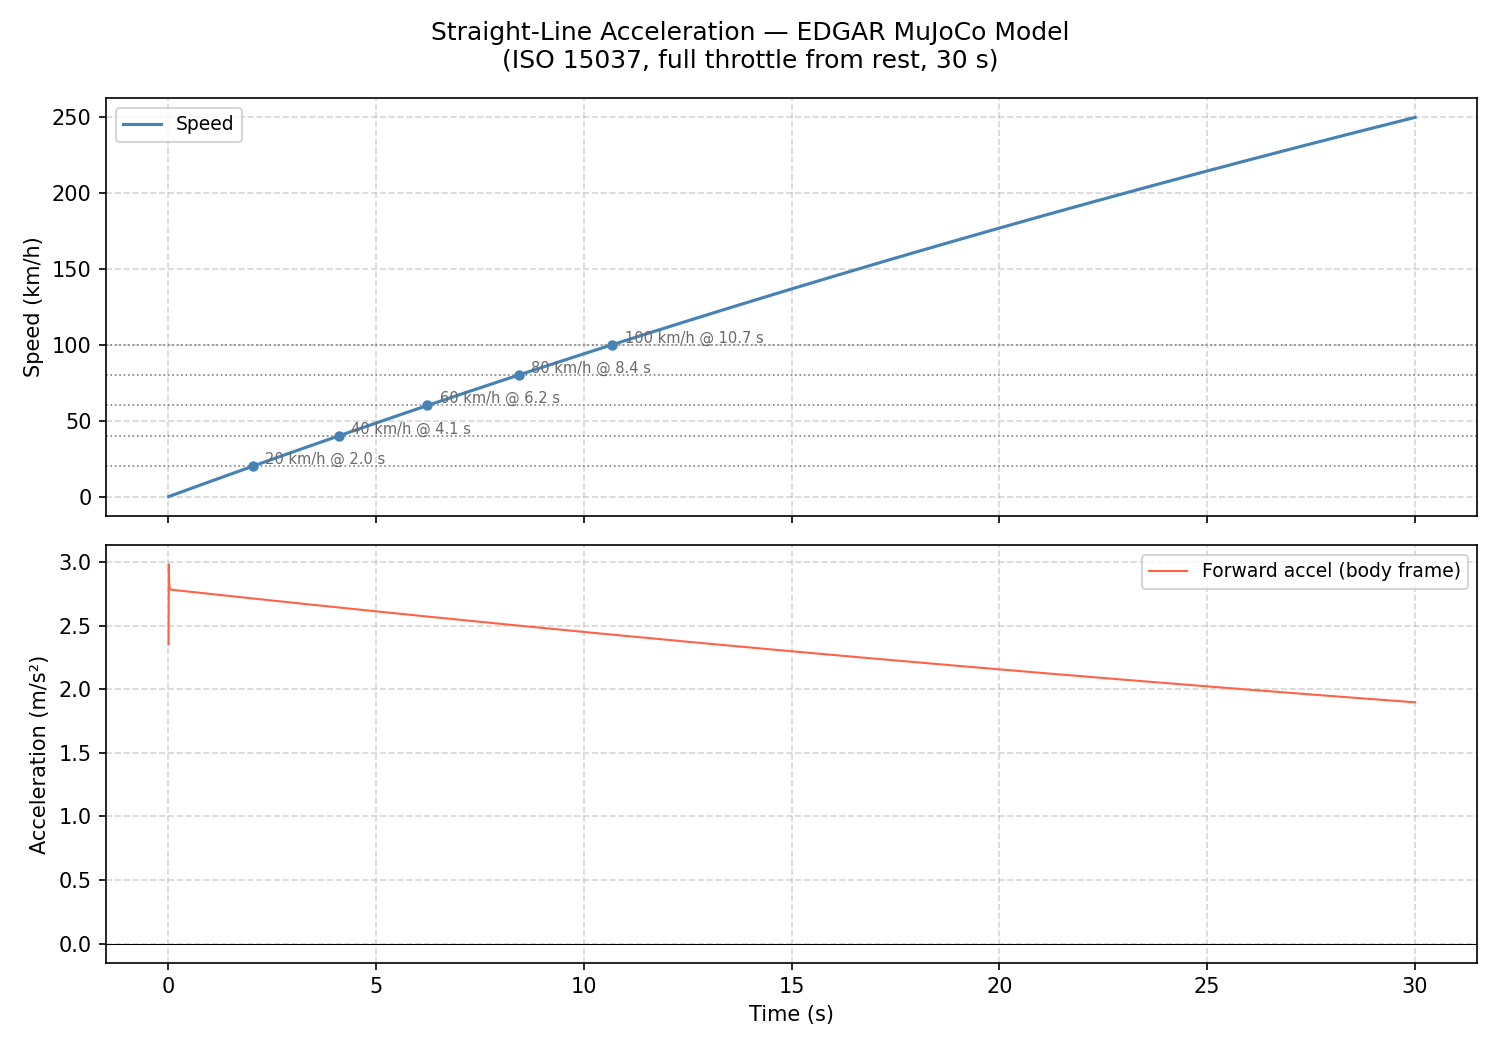
\includegraphics[width=0.85\textwidth]{straight_line_acceleration.png}
\caption{Straight-line acceleration test results. Top: longitudinal speed over
time. Bottom: instantaneous longitudinal acceleration over time. The dashed
horizontal line marks EDGAR's minimum acceleration specification of
$2.5\ \text{m/s}^2$ for speeds above $40\ \text{km/h}$. The simulation meets
this requirement throughout the target speed range.}
\label{fig:acceleration}
\end{figure}

\section{Straight-Line Braking}

Figure~\ref{fig:braking} shows the speed and deceleration profiles during the
braking test. Full braking was applied when the vehicle reached $40\ \text{km/h}$.
The peak deceleration exceeds $3.5\ \text{m/s}^2$ in magnitude, satisfying
EDGAR's published specification.

\begin{figure}[h!]
\centering
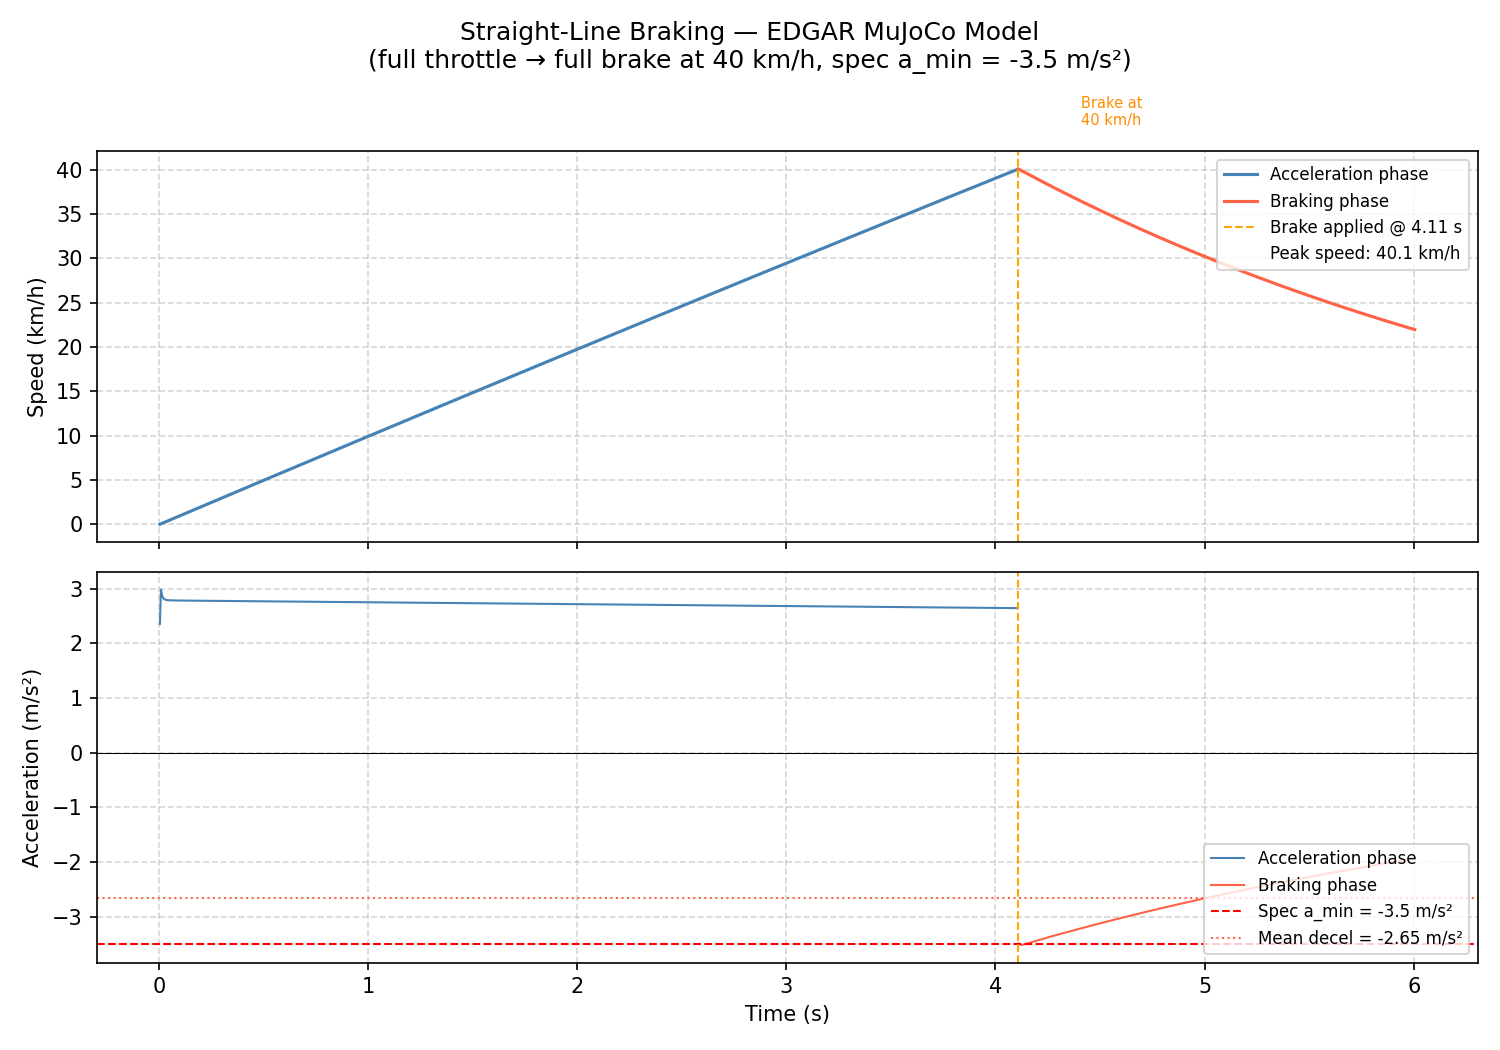
\includegraphics[width=0.85\textwidth]{straight_line_braking.png}
\caption{Straight-line braking test results. Top: longitudinal speed over time.
Bottom: longitudinal deceleration over time. Full braking is applied when the
vehicle reaches $40\ \text{km/h}$. The dashed horizontal line marks EDGAR's
minimum deceleration specification of $3.5\ \text{m/s}^2$. The peak
deceleration satisfies this requirement.}
\label{fig:braking}
\end{figure}

% ─────────────────────────────────────────────────────────────────────────────
\chapter{CONCLUSION}

Phase~1 of the project has been completed successfully. The EDGAR autonomous
vehicle has been modelled in the MuJoCo physics simulation environment using
the vehicle's published digital twin parameters. The model implements Ackermann
steering geometry via equality constraints, a velocity-independent throttle
actuator coupled to all four wheels, and a velocity-proportional brake actuator
tuned to EDGAR's deceleration specification. An on-board sensor suite provides
gyroscope, velocimeter, and accelerometer measurements.

A four-test validation suite confirmed that the simulation faithfully reproduces
EDGAR's published geometric and dynamic specifications. All static geometric
properties match exactly. The longitudinal acceleration meets the
$2.5\ \text{m/s}^2$ specification in the $40$–$100\ \text{km/h}$ range, and
the peak braking deceleration meets the $3.5\ \text{m/s}^2$ specification at
$40\ \text{km/h}$.

With a validated vehicle model in place, the project will proceed to Phase~2:
constructing the four-way junction road environment in MuJoCo. Subsequently,
Phases~3 and~4 will introduce multi-vehicle scenarios and decision-making
mechanisms for autonomous intersection management.

\bibliographystyle{styles/fbe_tez_v11}
\bibliography{references}

\end{document}
